\section{Experiments}
\label{sec:experiments}

We evaluate LLM-as-a-Verifier as a trajectory reward model (TRM) for test-time scaling across four benchmarks that span three domains: coding (Terminal-Bench V2~\citep{merrill_terminal-bench_2026}, SWE-Bench Verified~\citep{jimenez_swe-bench_2024}), robotics (RoboRewardBench~\citep{lee2026roboreward}), and medical (MedAgentBench~\citep{jiang2025virtual}). Across all four, we use the same protocol: a generation policy $\pi_\theta$ produces $N$ candidate trajectories per task, the verifier scores every pair using the probabilistic pivot tournament as described in Algorithm~\ref{alg:testtime}, and the trajectory with the highest normalized score is submitted. Unless otherwise noted, the verifier is run with granularity $G{=}20$, repeated evaluations $K{=}8$, and the three-criterion decomposition described in Section~\ref{sec:criteria}. Our method is training-free and plug-and-play: the same verification framework is applied across all four benchmarks without any per-domain fine-tuning. Overall results are summarized in Fig.~\ref{fig:teaser}, and per-benchmark headline numbers, including baseline accuracies, Pass@1, and oracle Pass@$N$, are reported in Table~\ref{tab:per-bench-headline}.

\begin{table}[h]
\centering
\caption{\textbf{Per-benchmark performance and gains from verification.} Baseline accuracies (left) are obtained under a fixed agent harness. On the same candidate pools, we report Pass@1, the oracle Pass@$N$ upper bound, and the accuracy achieved by LLM-as-a-Verifier (right). Our method consistently improves over Pass@1 and recovers a large portion of the oracle headroom, achieving state-of-the-art performance on each.}
\label{tab:per-bench-headline}
\small
\setlength{\tabcolsep}{4pt}
\begin{tabular}{l ccc ccc}
\toprule
 & \multicolumn{3}{c}{\textbf{Baseline models (accuracy)}} & \multicolumn{3}{c}{\textbf{LLM-as-a-Verifier}} \\
\cmidrule(lr){2-4}\cmidrule(lr){5-7}
Benchmark & \#1 & \#2 & \#3 & Pass@1 & Oracle & \textbf{Ours} \\
\midrule
Terminal-Bench V2  & GPT-5.5 (84.7\%)        & Opus 4.7 (80.2\%) & G3.1 Pro (80.2\%) & 83.1\% & 92.1\% & \textbf{86.5\%} \\
SWE-Bench Verified & Opus 4.5 (76.8\%)       & G3 Flash (75.8\%)        & M2.5 (75.8\%)           & 76.1\% & 84.4\% & \textbf{78.2\%} \\
MedAgentBench      & Opus 4.8 (70.2\%)       & G3.5 Flash (66.3\%)        & GPT-5.5 (65.1\%)       & 70.2\% & 75.0\% & \textbf{73.3\%} \\
\bottomrule
\end{tabular}
\end{table}

\subsection{Terminal-Bench V2}
\label{sec:terminal}

Terminal-Bench V2~\citep{merrill_terminal-bench_2026} measures an agent's proficiency in shell-based environments across long-horizon tasks that require multi-step reasoning, file manipulation, and recovery from failed tool calls. The benchmark is particularly difficult for verifiers because many trajectories produce syntactically plausible but incorrect terminal states. We use Capy~\citep{capy} as the scaffold and sample $N{=}5$ trajectories per task from GPT-5.5; Gemini 2.5 Flash serves as the verifier. The Pass@1 of GPT-5.5 under Capy is $83.1\%$, and the oracle Pass@5 upper bound on this candidate pool is $92.1\%$. LLM-as-a-Verifier improves the accuracy from $83.1\%$ to $\mathbf{86.5\%}$, surpassing Claude Mythos + Terminus-2~\citep{noauthor_terminal-benchterminal_benchagentsterminus_2_nodate} ($82.0\%$), GPT-5.5 + NexAU-AHE ($84.7\%$), Claude Opus 4.7 + WOZCODE ($80.2\%$), and Gemini 3.1 Pro + TongAgents ($80.2\%$) and setting a new state of the art on Terminal-Bench V2.\footnote{Baseline accuracies are extracted from the official Terminal-Bench~V2 and SWE-Bench Verified leaderboard.} We further show that these gains are not tied to a specific harness. For additional generalization results on Terminus-2 and Terminus-Kira, refer to Appendix~\ref{app:harness}.

\subsection{SWE-Bench Verified}
\label{sec:swebench}

SWE-Bench Verified~\citep{jimenez_swe-bench_2024} is a human-curated subset of 500 real-world GitHub issues where each task requires an agent to produce a patch that resolves the issue and passes the maintainer's hidden test suite. It stresses long-context reasoning, cross-file edits, and compliance with an existing codebase. We use mini-swe-agent as the scaffold and, in contrast to the homogeneous proposal pool used on Terminal-Bench, draw a heterogeneous pool of $N{=}3$ candidates per task by sampling one trajectory each from Claude Opus 4.5, Gemini 3 Flash, and MiniMax M2.5. Gemini 2.5 Flash again serves as the verifier. The mean Pass@1 across this candidate pool is $76.1\%$ and the oracle Pass@3 upper bound is $84.4\%$. LLM-as-a-Verifier achieves $\mathbf{78.2\%}$ on SWE-Bench Verified, outperforming Claude Opus 4.5 ($76.8\%$), Gemini 3 Flash ($75.8\%$), and MiniMax M2.5 ($75.8\%$). These results highlight the verifier's ability to select the strongest trajectory from a diverse set of candidates produced by different model families.

\subsection{RoboRewardBench}
\label{sec:roboreward}

\begin{wraptable}{r}{0.42\textwidth}
\vspace{-\baselineskip}
\centering
\caption{\textbf{Preference accuracy on RoboRewardBench.} LLM-as-a-Verifier outperforms trained robotics reward models.}
\label{tab:roboreward}
\small
\setlength{\tabcolsep}{6pt}
\begin{tabular}{lc}
\toprule
Method & Accuracy (\%) \\
\midrule
TOPReward                  & 74.7 \\
Robometer-4B               & 78.8 \\
RoboReward-8B              & 81.4 \\
LLM-as-a-Judge (Discrete)  & 70.8 \\
\textbf{LLM-as-a-Verifier (Ours)} & \textbf{87.4} \\
\bottomrule
\end{tabular}
\vspace{-\baselineskip}
\end{wraptable}

RoboRewardBench~\citep{lee2026roboreward} evaluates reward models on robotic manipulation trajectories. Following~\citet{liang2026robometer}, we curate pairs of rollout videos that follow the same natural-language instruction but make different amounts of progress; the reward model must output a preference indicating which rollout makes more progress. Unlike the coding and clinical benchmarks, inputs here are multi-frame videos, so the verifier must integrate visual context across frames to reason about physical progress toward the goal. We use Qwen 3.6 35B as the base VLM verifier and apply the same probabilistic formulation (Eq.~1) over scoring tokens extracted from the VLM's logits, with granularity $G{=}20$ and $K{=}8$ repeated verifications. We evaluate on 500 randomly sampled trajectory pairs from the RoboRewardBench and compare against (i)~a discrete LLM-as-a-Judge baseline using the same VLM, (ii)~reward models specifically trained on robotics data---RoboReward-8B (trained on $\sim$45k episodes) and Robometer-4B (trained on $\sim$1M comparisons), and (iii)~TOPReward~\cite{chen2026topreward} (Qwen 3.6). As shown in Table~\ref{tab:roboreward} and Appendix~\ref{app:roboreward}, LLM-as-a-Verifier achieves $\mathbf{87.4\%}$ preference accuracy, outperforming the discrete LLM-as-a-Judge baseline ($70.8\%$), RoboReward-8B ($81.4\%$), Robometer-4B \cite{liang2026robometer} ($78.8\%$), and TOPReward (74.7\%), despite being applied zero-shot and without any fine-tuning. We also evaluate on RoboRewardBench by measuring the Mean Absolute Error (MAE) between predicted rewards and human annotations. As shown in Table~\ref{tab:roboreward-mae}, using the continuous reward formulation in Eq.~\ref{eq:main} together with $K{=}8$ repeated evaluations substantially improves alignment with human judgments, reducing the MAE from $1.11$ to $\mathbf{0.72}$.

\begin{table}[h]
\centering
\caption{\textbf{Evaluation on RoboRewardBench against human annotations.} We report Mean Absolute Error (MAE; lower is better) between human labels and predicted rewards. LLM-as-a-Verifier uses continuous rewards ($K{=}8$), whereas the baseline extracts discrete scores from the model.}
\label{tab:roboreward-mae}
\small
\setlength{\tabcolsep}{8pt}
\begin{tabular}{lc}
\toprule
Models & RoboRewardBench MAE ($\downarrow$) \\
\midrule
RoboReward 8B                          & 1.11 \\
\textbf{RoboReward 8B + LLM-as-a-Verifier} & \textbf{0.72} \\
\bottomrule
\end{tabular}
\end{table}

\subsection{MedAgentBench}
MedAgentBench~\citep{jiang2025virtual} evaluates LLM agents on medical tasks that involve patient information retrieval, guideline lookup, and multi-step tool use in a simulated electronic health records (EHR) environment. It covers a regime where ground-truth trajectory checkers are expensive to construct and where verification errors carry real safety consequences, making it a natural stress test for general-purpose verifiers. We use the AgentBench harness and sample $N{=}5$ trajectories per task from Claude Opus 4.8, then apply the same verification procedure. The Pass@1 of Claude Opus 4.8 on this pool is $70.2\%$ and LLM-as-a-Verifier achieves $\mathbf{73.3\%}$, outperforming Opus 4.8 ($70.2\%$), Gemini 3.5 Flash ($66.3\%$), and GPT-5.5 ($65.1\%$).

\begin{figure}[t!]
    \centering
    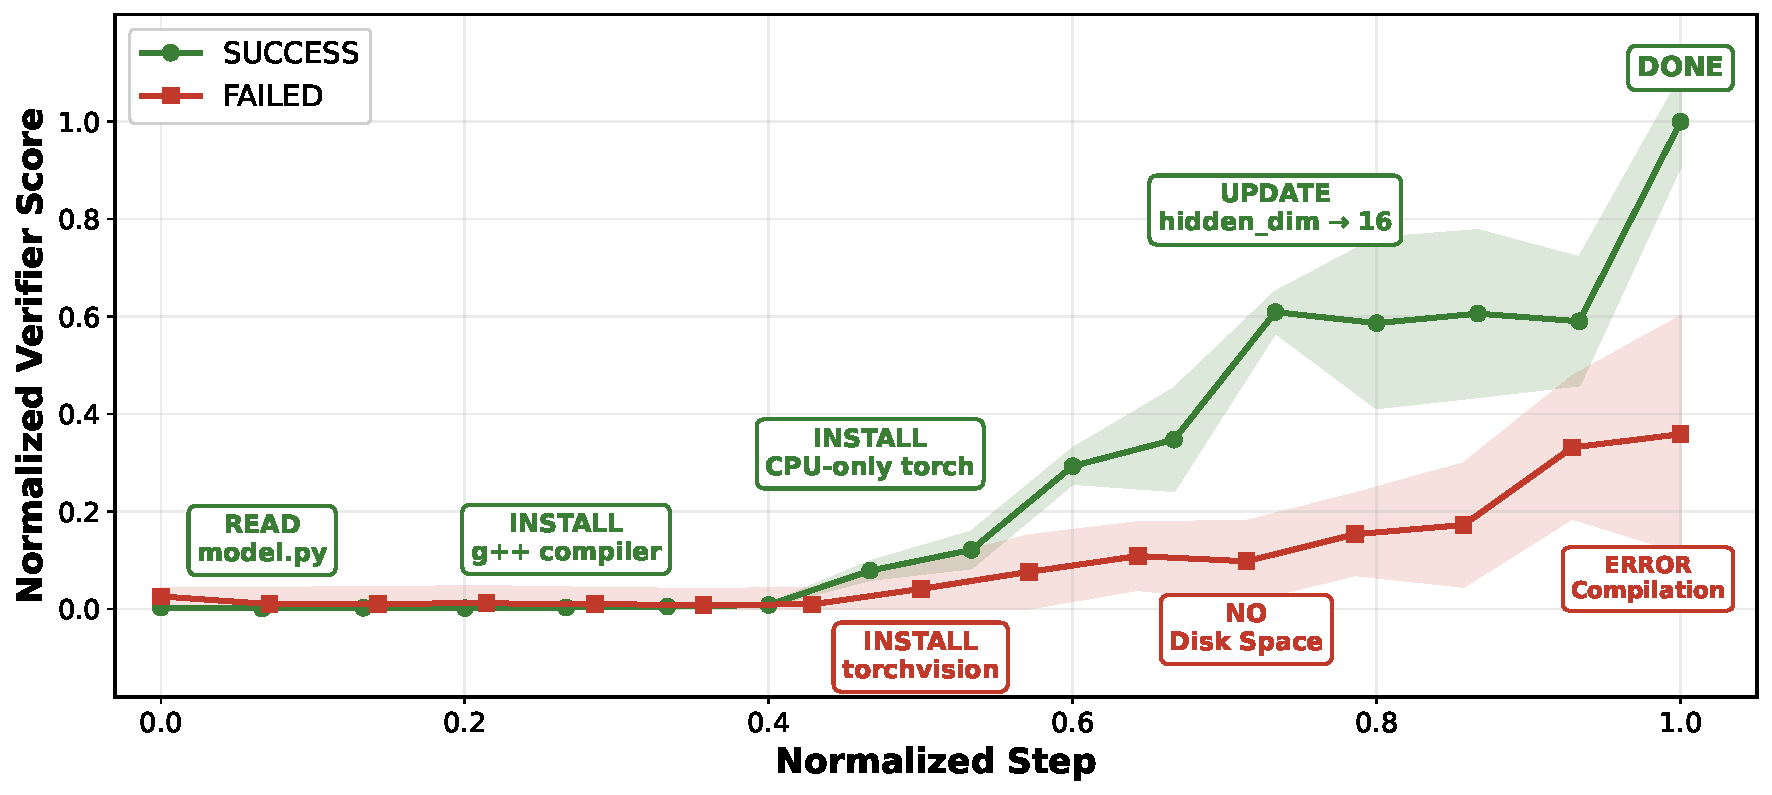
\includegraphics[width=0.98\linewidth]{figures/voc_pytorch_model_cli.pdf}
    \caption{We observe a strong correlation between the chronological progression of code generation steps and the scores from LLM-as-a-Verifier. The example task above requires the agent to run MNIST inference. The successful trajectory follows a coherent sequence of events---\emph{Read \texttt{model.py} $\rightarrow$ Install g++ compiler $\rightarrow$ Install CPU-only torch $\rightarrow$ Update \texttt{hidden\_dim}} $\rightarrow$ DONE and exhibits consistently increasing verifier scores. In contrast, the failed trajectory is characterized by erroneous behaviors---it unnecessarily installs the large \texttt{torchvision} package, which exhausts the available disk space and hits a compilation error---resulting in significantly lower scores. Results are shown for the \texttt{pytorch-model-cli} task from Terminal-Bench V2, using Gemini 2.5 Pro with Terminus 2 and Gemini 2.5 Flash as the verifier.}
    \label{fig:voc-counterfactual-code}
\end{figure}

\section{Fine-grained Verifier Signals as a Proxy for Task Progress}
\label{sec:progress}

Beyond selecting the best trajectory, the fine-grained signal produced by LLM-as-a-Verifier can serve as a scalar proxy for how far an agent has progressed through a task. We quantify this using the \emph{Value-Order Correlation} (VOC), the Spearman rank correlation between the chronological index of a step and the verifier's predicted value for the prefix ending at that step, following \citet{ICLR2025_54854cf1}. Intuitively, a verifier that tracks task progress should assign monotonically higher scores to later prefixes of a successful rollout, yielding $\mathrm{VOC}\to 1$, and should remain robust to failure modes such as getting stuck or regressing.
\begin{equation}
\mathrm{VOC} = \mathrm{rank\text{-}correlation}\!\left(
\mathrm{argsort}(s_{t_1}, s_{t_2}, \cdots, s_{t_K}),
(t_1, t_2, \cdots, t_K)
\right).
\end{equation}


\paragraph{VOC on code generation.} On Terminal-Bench V2, we measure VOC between the chronological step of each agent action and the verifier's score on the corresponding trajectory prefix. LLM-as-a-Verifier produces consistently increasing scores on successful rollouts while remaining largely flat on trajectories that stall or drift toward failure, allowing the same scalar to serve as both a progress measure and an early-warning signal. Figure~\ref{fig:voc-counterfactual-code} illustrates this on the \texttt{pytorch-model-cli} task, where the successful run's score rises monotonically while the failed run's stays low. This dual use motivates our Claude Code and Codex extensions, which surface the live verifier score to the user so that long-running agentic jobs can be monitored, paused, or rolled back before they commit broken state to disk. Across 500 (success, failure) pairs drawn from Terminal-Bench V2 runs, the verifier (Gemini 2.5 Flash, $G{=}20$) attains Spearman VOC $0.848$ on successful trajectories and $0.769$ on failed ones (full numbers reported in Table~\ref{tab:voc-terminal-by-outcome}). The code-generation VOC numbers indicate that the fine-grained signal produced by LLM-as-a-Verifier is not merely a better ranker but a calibrated estimator of task progress, opening a path toward safer real-world deployment of autonomous agents.

\begin{table}[h]
    \centering
    \begin{tabular}{lc}
        \toprule
        \textbf{Trajectory outcome} & \textbf{Spearman VOC (rank correlation)} \\
        \midrule
        Successful                                & $0.848 \pm 0.012$ \\
        Failed                                    & $0.769 \pm 0.016$ \\
        \midrule
        Success $-$ Failed (gap)                  & $+0.079$          \\
        \bottomrule
    \end{tabular}
\caption{\textbf{Value-Order Correlation by trajectory outcome on Terminal-Bench V2.}
Mean Spearman rank correlation between step index and verifier progress score, computed over 500 randomly sampled trajectories from Terminal-Bench V2. The verifier (Gemini 2.5 Flash, $G{=}20$) exhibits near-monotonic progress for successful trajectories, while failed rollouts show weaker correlation, indicating limited or inconsistent progress. We observe a $0.08$ Spearman gap between successful and failed trajectories generated by the same agent backbone on the same task.}
    \label{tab:voc-terminal-by-outcome}
\end{table}

\paragraph{VOC on robotics.} We compute VOC over 500 trajectories from the held-out RoboReward dataset. As shown in Table~\ref{tab:voc-roboreward}, LLM-as-a-Verifier (Qwen 3.6, $K{=}5$, $G{=}20$) attains $\mathbf{0.966}$, substantially exceeding RoboReward-8B ($0.877$), Robometer-4B ($0.780$), and TOPReward ($0.565$). Qualitatively, TOPReward tends to saturate at $P(\texttt{True}){=}1.0$ almost immediately and therefore loses the ability to discriminate mid-trajectory progress when a rollout eventually fails, whereas our expectation over the full scoring distribution preserves a smooth, chronologically-aligned signal throughout the episode.

\begin{table}[h]
    \centering
    \begin{tabular}{lc}
        \toprule
        \textbf{Method} & \textbf{Spearman VOC (rank correlation)} \\
        \midrule
        LLM-as-a-Verifier (Qwen 3.6 35B, 5 reps, 20 granularity) & \textbf{0.966} \\
        RoboReward-8B & 0.877 \\
        Robometer-4B & 0.780 \\
        TOPReward (Qwen 3.6, $P(\texttt{true})$) & 0.565 \\
        \bottomrule
    \end{tabular}
    \caption{\textbf{Value-Order Correlation on 500 trajectories from RoboRewardBench.} LLM-as-a-Verifier with $K{=}5$ repeated evaluations and $G{=}20$ scoring granularity attains the highest rank-correlation between the chronological step index and the verifier's predicted progress score.}
    \label{tab:voc-roboreward}
\end{table}

\paragraph{Coding Agent Extension} To demonstrate the applicability of LLM-as-a-Verifier to real-world coding agents, we develop \textbf{\textit{TurboAgent}}, a drop-in extension for Claude Code and other OpenAI-API compatible clients. TurboAgent operates as an inference-time proxy that transparently sits between the client and the LLM provider, requiring no modifications to either the underlying agent harness or the backend model. The proxy design also allows TurboAgent to be plugged transparently into existing benchmarks such as Terminal-Bench~\citep{merrill_terminal-bench_2026}. For each request, it dispatches $N$ candidate trajectories to the backend model in parallel and selects the best response using the proposed \emph{Probabilistic Pivot Tournament} (PPT). Beyond verification, TurboAgent also provides a web-based interface for visualizing verifier outputs and monitoring agent progress in real time.

\section{Dense Reward for Reinforcement Learning}
\label{sec:rl}


\begin{figure}[h!]
    \centering
    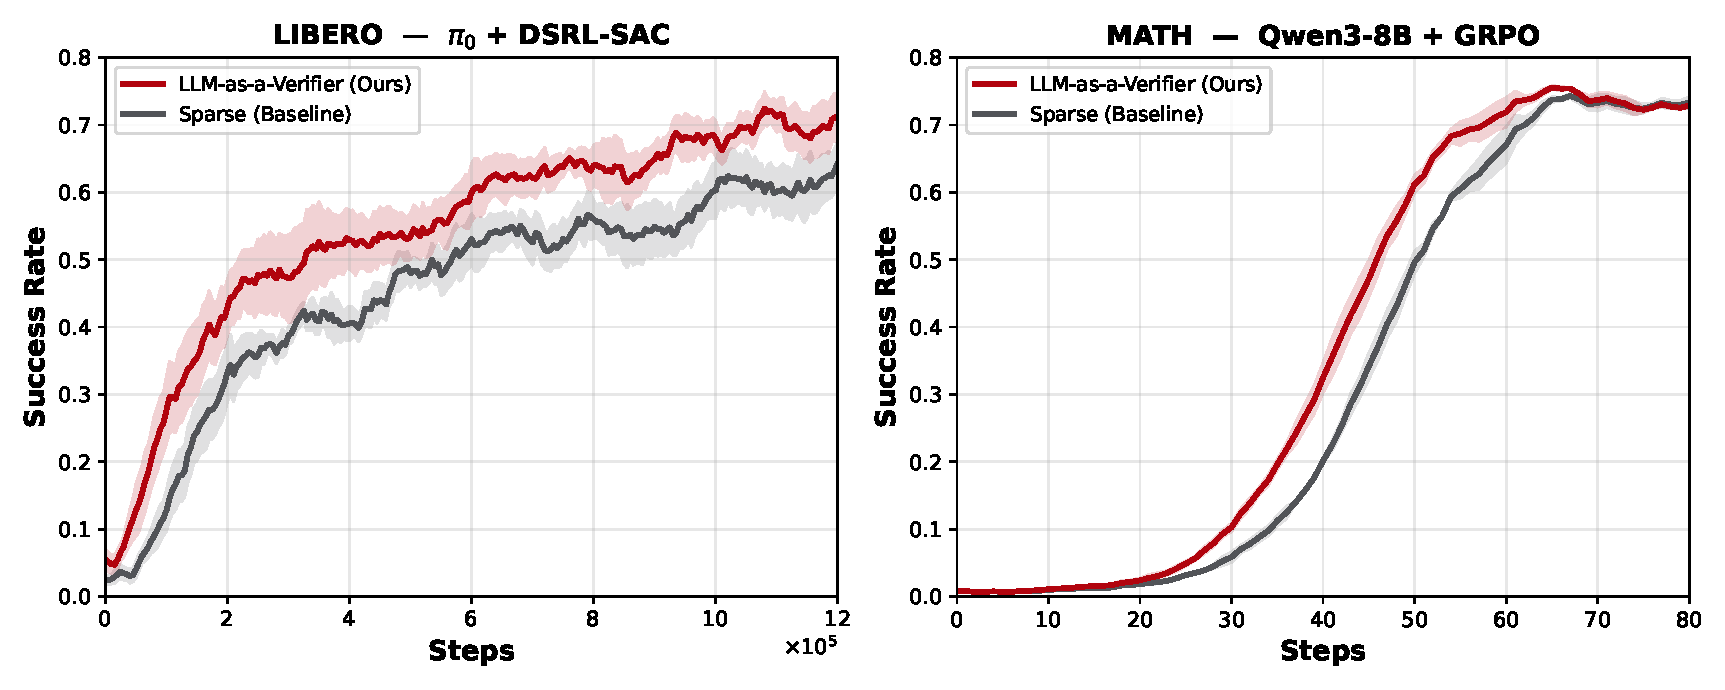
\includegraphics[width=\linewidth]{figures/combined_libero_math.pdf}
    \caption{\textbf{LLM-as-a-Verifier improves RL sample efficiency.} Success rate versus training steps for off-policy (left) and on-policy (right) reinforcement learning, comparing sparse-reward baselines with dense rewards from LLM-as-a-Verifier. \textbf{Left:} A $\pi_0$ policy fine-tuned on the LIBERO \texttt{ketchup} task with DSRL-SAC. The verifier progress reward (Eq.~\ref{eq:rl-sac}) achieves the same success rate using $\approx1.8\times$ fewer environment steps and reaches a higher final success rate ($0.76$ vs.\ $0.69$). \textbf{Right:} Qwen3-8B fine-tuned on MATH with GRPO. The verifier reasoning reward (Eq.~\ref{eq:rl-grpo}) improves sample efficiency by $\approx1.1\times$. Results are averaged over multiple seeds (LIBERO $n{=}5$, MATH $n{=}3$).} 
    \label{fig:rl-sample-efficiency}
\end{figure}

The progress signal from the previous section also helps remediate a long-standing difficulty in reinforcement learning (RL): the \emph{credit assignment problem}. We show that the fine-grained score of LLM-as-a-Verifier (Eq.~\ref{eq:main}) is a drop-in dense reward for both off-policy and on-policy RL, improving sample efficiency without any reward-model training or environment-specific shaping.

\paragraph{Off-policy RL: dense progress rewards for DSRL-SAC.} We fine-tune the $\pi_0$~\citep{black2026pi0visionlanguageactionflowmodel} vision–language–action model on LIBERO with DSRL using Soft Actor–Critic (SAC). At the end of each rollout we query the VLM verifier with the task instruction $x$ and a uniformly sub-sampled sequence of rendered frames, obtaining a per-step progress curve $\rho_t = R\!\left(x, \tau_{1:t}\right)\in[0,1]$. We then relabel the rollout with the shaped reward:
\begin{equation}
r_t \;=\; r^{\text{env}}_t \;+\; \lambda\,\rho_t,
\label{eq:rl-sac}
\end{equation}
store the relabeled transitions $(s_t, a_t, r_t, s_{t+1})$ in the replay buffer $\mathcal{D}$, and train the SAC critic on the relabeled returns sampled from $\mathcal{D}$. The coefficient $\lambda$ trades off environment and verifier rewards. Because shaping is applied offline to stored trajectories and leaves the SAC objective untouched, it adds dense intermediate signals at no additional algorithmic cost.

\paragraph{On-policy RL: dense reasoning rewards for GRPO.} We fine-tune Qwen3-8B~\citep{yang2025qwen3} on MATH using Group Relative Policy Optimization (GRPO)~\citep{deepseek-ai_deepseek-r1_2025}, which samples a group of $G$ responses $\{y_i\}_{i=1}^{G}$ for each prompt $x$ and estimates each response's advantage relative to the group. During the early stages of training, it is common for all sampled responses to produce incorrect final answers, causing the group-relative advantage to collapse to zero and yielding no gradient. LLM-as-a-Verifier mitigates this issue by evaluating the reasoning trace of each completion using the probabilistic pivot tournament (Eq.~\ref{eq:pref}), assigning each response a normalized preference score $\bar{R}_i \in [0,1]$ that captures fine-grained differences in reasoning quality even when the final answers are identical. We incorporate this verifier-derived score into the standard correctness and format reward with weight $\beta$:
\begin{equation}
r_i
=
r_{\mathrm{correct},i}
+
r_{\mathrm{format},i}
+
\beta\, r_{\mathrm{reasoning},i}.
\label{eq:rl-grpo}
\end{equation}


\paragraph{Empirical findings.} Across both regimes, dense verifier rewards improve sample efficiency over the sparse baselines
%under an identical policy, optimizer, and seed 
(Fig.~\ref{fig:rl-sample-efficiency}). We quantify sample efficiency as the ratio of training steps the sparse baseline requires to reach a target success rate to the steps our dense reward requires. On LIBERO, shaping a $\pi_0$ policy trained with DSRL-SAC reaches a matched success rate in substantially fewer environment steps--- $\mathbf{1.8\times}$ higher sample efficiency across success-rate targets from $0.2$ to $0.6$---while also attaining a higher final success rate ($0.76$ vs.\ $0.69$). On MATH, augmenting GRPO with the reasoning reward gives a smaller but consistent gain of $\approx\mathbf{1.1\times}$ (a $\sim\!10\%$ reduction in the optimizer steps needed to reach a matched accuracy). We report reward-shaping hyperparameters and additional ablations in Appendix~\ref{app:rl}.